% generic-discrimination.tex
%
% Generic discrimination
% Fritz Henglein, Department of Computer Science, University of Copenhagen (DIKU)
% Advanced Programming, DIKU, 2026-10-20
%
% Based on the slides presented at SSGEP (Summer School on Generic and
% Effectful Programming), Oxford, 2015-07-06, whose Beamer source was
% reconstructed from the PDF; typos fixed, Haskell code set in shaded boxes
% with syntax coloring (listings + tcolorbox).
% Compile with:   pdflatex generic-discrimination.tex
%
% The University of Copenhagen slide design is reproduced here without the
% original theme files.  The two page backgrounds (title page and ordinary
% slides) and the five performance charts were extracted from the 2015 PDF
% into figures/; the colors, fonts and placements below are taken from it as
% well.

\documentclass{beamer}

% ---------------------------------------------------------------------------
% KU look and feel
% ---------------------------------------------------------------------------
\useinnertheme[shadow=true]{rounded}

\definecolor{kugreen}{RGB}{50,93,61}
\usecolortheme[named=kugreen]{structure}
\setbeamercolor{frametitle}{fg=kugreen}
\setbeamercolor{title}{fg=white,bg=kugreen}
\setbeamercolor{block title}{fg=white,bg=kugreen}
\setbeamercolor{block body}{fg=black,bg=kugreen!25}

\setbeamerfont{frametitle}{size=\Large,series=\bfseries}
\setbeamerfont{block title}{size=\normalsize}
\setbeamertemplate{navigation symbols}{}

% ---------------------------------------------------------------------------
% Haskell code
%   * Display code: environment haskell, a listing in a rounded, lightly
%     shaded box as wide as the code.  Optional argument: further listings
%     options, e.g. \begin{haskell}[style=long] (smaller type) for code
%     with long lines.
%   * Inline code: \lstinline|...|.
% Frames that contain code must be [fragile].  The code font is DejaVu Sans
% Mono (the font Menlo is based on) where installed, else Computer Modern
% Typewriter.  Syntax colors follow GitHub's light theme: keywords bold red,
% types and data constructors blue.
% ---------------------------------------------------------------------------
\IfFileExists{DejaVuSansMono.sty}{\usepackage[scaled=0.85]{DejaVuSansMono}}{}
\usepackage{listings}
\usepackage{tcolorbox}
\tcbuselibrary{listings}

\definecolor{codebackground}{HTML}{F6F8FA}
\definecolor{codeframe}{HTML}{D0D7DE}
\definecolor{codekeyword}{HTML}{CF222E}
\definecolor{codetype}{HTML}{0550AE}
\definecolor{codestring}{HTML}{0A3069}
\definecolor{codecomment}{HTML}{6E7781}

\lstset{%
  language=Haskell,
  % reserved words (the Haskell definition of listings also lists most
  % Prelude functions as keywords)
  keywords={case,class,data,default,deriving,do,else,foreign,if,import,in,
            infix,infixl,infixr,instance,let,module,newtype,of,then,type,
            where},
  % types and data constructors -- add new ones here
  keywords=[2]{Bool,Char,Double,Either,Eq,Equiv,False,Float,IO,IOArray,
               Int,Integer,Just,Left,Maybe,Nothing,Ord,Order,Ordering,Ref,
               Right,Show,String,True,
               Nat,Triv,SumL,PairL,MapO,Inv,BagO,SetO,R,
               NatE,TrivE,SumE,ProdE,MapE,ListE,BagE,SetE},
  basicstyle=\upshape\ttfamily,
  keywordstyle={\color{codekeyword}\bfseries},
  keywordstyle=[2]{\color{codetype}},
  commentstyle={\color{codecomment}\itshape},
  stringstyle={\color{codestring}},
  columns=fullflexible,
  keepspaces=true,
  upquote=true,
  showstringspaces=false}
\lstdefinestyle{display}{basicstyle=\upshape\ttfamily\small}
\lstdefinestyle{long}{basicstyle=\upshape\ttfamily\footnotesize}

\newtcblisting{haskell}[1][]{%
  listing only, hbox,
  colback=codebackground, colframe=codeframe,
  boxrule=0.5pt, arc=2pt, boxsep=0pt,
  left=4pt, right=6pt, top=2pt, bottom=2pt,
  enlarge left by=-4.5pt,
  before skip=4pt, after skip=4pt,
  listing options={style=display,#1}}

% Page backgrounds (KU header bar, seal and dots); the title page has its own.
\newcommand{\kubackground}[1]{%
  \setbeamertemplate{background}{%
    \includegraphics[width=\paperwidth,height=\paperheight]{#1}}}
\kubackground{figures/ku-background}

% Frame title: bold, green, left-aligned just below the KU header bar.  The
% lengths below (and those for the footline and title page) reproduce the
% placement in the original PDF.
\newlength{\kutitletop}     \setlength{\kutitletop}{16.54pt}
\newlength{\kutitleindent}  \setlength{\kutitleindent}{14.54pt}
\newlength{\kutitlebottom}  \setlength{\kutitlebottom}{-6.61pt}
\setbeamertemplate{frametitle}{%
  \vskip\kutitletop
  \begin{beamercolorbox}[wd=\paperwidth,leftskip=\kutitleindent,
                         rightskip=0pt plus 1fil]{frametitle}%
    \usebeamerfont{frametitle}\strut\insertframetitle\strut\par
  \end{beamercolorbox}%
  \vskip\kutitlebottom}

% Footline: just the slide number, in the bottom left corner.
\newlength{\kufootheight}   \setlength{\kufootheight}{13.92pt}
\setbeamertemplate{footline}{%
  \vbox to\kufootheight{%
    \vfil
    \hbox to\paperwidth{\hskip5pt\usebeamerfont{footline}\tiny
      \insertframenumber\hfil}%
    \vskip10pt}}

% Title page: rounded green title box near the top, then author, institute
% and date (occasion); the bottom right is taken by the painting.
\newlength{\kutitlepagetop}  \setlength{\kutitlepagetop}{39.45pt}
\newlength{\kudateskip}      \setlength{\kudateskip}{2pt}
\setbeamertemplate{title page}{%
  \vskip\kutitlepagetop
  \begingroup
    \centering
    \begin{beamercolorbox}[sep=4pt,center,colsep=-4bp,rounded=true,
                           shadow=true]{title}
      \usebeamerfont{title}\inserttitle\par
    \end{beamercolorbox}%
    \vskip1em\par
    \begin{beamercolorbox}[sep=8pt,center]{author}
      \usebeamerfont{author}\insertauthor
    \end{beamercolorbox}
    \begin{beamercolorbox}[sep=8pt,center]{institute}
      \usebeamerfont{institute}\insertinstitute
    \end{beamercolorbox}
    \vskip\kudateskip
    \begin{beamercolorbox}[sep=8pt,center]{date}
      \usebeamerfont{date}\insertdate
    \end{beamercolorbox}
  \endgroup
  \vskip0pt plus 1filll}

% ---------------------------------------------------------------------------
\newtheorem{proposition}[theorem]{Proposition}

\title{Generic discrimination}
\author{Fritz Henglein\\ \texttt{henglein@diku.dk}}
\institute{Department of Computer Science\\ University of Copenhagen\\ (DIKU)}
\date{Advanced Programming, DIKU, 2026-10-20\\[0.5ex]
  {\scriptsize Based on presentation at Summer School on\\
    Generic Programming, Oxford U., 2015-07-06\par}}

\begin{document}

% ===========================================================================
{\kubackground{figures/ku-background-title}
\begin{frame}[plain]
  \titlepage
\end{frame}
}

% ===========================================================================
\begin{frame}{Some simple problems}
  \begin{itemize}
  \item Given a list of pointers, \emph{how many unique elements} does it
    contain?
  \item Given a list of pointers, what are its \emph{unique elements}?
  \item Given a list of pointer lists, what are its \emph{unique pointer
      lists}?
  \item Given a list of pointer sets (given as lists considered equal modulo
    permutations and duplicates), what are its \emph{unique pointer sets}?
  \item How efficient are your solutions?
  \item Do they allow copying garbage collection?
  \end{itemize}
\end{frame}

\begin{frame}{Great speed, no abstraction}
  The C and Java solution:
  \begin{itemize}
  \item Convert pointers to numbers (casting, hashing)
  \item Use address arithmetic and table lookups.
  \end{itemize}
  Consequences:
  \begin{itemize}
  \item Potentially nondeterministic program behavior:
    \texttt{ptr = new ... ; if ptr < 4000 then ...}
  \item No data abstraction: Cannot change implementation, impedes garbage
    collection.
  \end{itemize}
\end{frame}

\begin{frame}{Great abstraction, no speed}
  The ML solution:
  \begin{itemize}
  \item Abstract pointers (references): Allow only equality testing, lookup,
    allocation, update on pointers.
  \item Use pairwise comparisons.
  \end{itemize}
\end{frame}

\begin{frame}{Great abstraction, no speed}
  The ML solution:
  \begin{itemize}
  \item Abstract pointers (references): Allow only equality testing, lookup,
    allocation, update on pointers.
  \item Use pairwise comparisons.
  \end{itemize}
  Consequence:
  \begin{theorem}
    Determining the number of unique elements in a list of $n$ ML references
    takes $\Omega(n^2)$ equality tests.
  \end{theorem}
\end{frame}

\begin{frame}{Have your cake and eat it too?}
  Question: Can you sort and partition
  \begin{itemize}
  \item \emph{generically}: user-defined orders/equivalences;
  \item \emph{fully abstractly}: pairwise comparisons determine output;
  \item \emph{scalably}: worst-case \emph{linear}
    time\footnote{for standard and many other orders/equivalences}
  \end{itemize}
  expressed with very short and simple program code?

  \vspace{1cm}
  Answer: Yes
\end{frame}

\begin{frame}[fragile]{Great abstraction, great speed}
\begin{haskell}
part :: Equiv k -> [k] -> [[k]]

numUniqElems ps = length (part eqRef ps)
uniqElems ps = [ head b | b <- part eqRef ps ]
uniqPtrLists pss = [ head b | b <- part (listE eqRef) pss]
uniqPtrSets pss = [ head b | b <- part (SetE eqRef) pss ]
\end{haskell}
  \begin{itemize}
  \item Worst-case linear time\\
    ($= O(\textrm{number of pointer occurrences})$)
  \item Same order of pointers before and after garbage collection ($=$
    \emph{as if} using only equality tests to compute result)
  \end{itemize}
\end{frame}

\begin{frame}[fragile]{Key ingredient: Discriminator}
  Provide $n$-ary ``comparison'' function
\begin{haskell}
discRef :: [(Ref a, v)] -> [[v]]
\end{haskell}
  to data type instead of binary comparison function
\begin{haskell}
== :: Ref a -> Ref a -> Bool
\end{haskell}
  \begin{itemize}
  \item Fully abstract: Only pairwise equality can be ``observed'' through
    \lstinline|discRef| (like having only \lstinline|==|).
  \item Asymptotically optimal performance: $O(n)$ worst-case time (like
    treating pointers---internally---as numbers).
  \end{itemize}
\end{frame}

\begin{frame}{Generic discrimination: Method}
  \begin{itemize}
  \item Expressive \emph{domain-specific language} for defining orders and
    equivalences \emph{compositionally}.
  \item Inherently efficient (usually linear-time and fully abstract)
    \emph{discriminators} by structural recursion (``generically'') on order
    and equivalence representations.
  \item Partitioning, sorted partitioning, sorting, joining functions, etc.,
    as \emph{applications} of discriminators.
  \end{itemize}
\end{frame}

\begin{frame}[fragile]{Example: Word occurrences}
  Word occurrences, alphabetically sorted:
\begin{haskell}
occsO :: [(String, Int)] -> [[Int]]
occsO = sdisc ordString8
\end{haskell}
  Word occurrences, in order of occurrence in input
\begin{haskell}
occsE :: [(String, Int)] -> [[Int]]
occsE = disc eqString8
\end{haskell}
\end{frame}

\begin{frame}[fragile]{Example: Word occurrences, case insensitive}
  Definition of alphabetic order, but case-insensitive:
\begin{haskell}
ordString8Ins :: Order String
ordString8Ins = listL (MapO toUpper ordChar8)
\end{haskell}
  Word occurrences, case insensitive, alphabetically sorted:
\begin{haskell}
occsCaseInsO :: [(String, Int)] -> [[Int]]
occsCaseInsO = sdisc ordString8Ins
\end{haskell}
  Word occurrences, case insensitive, order of occurrence in input:
\begin{haskell}
occsCaseInsE :: [(String, Int)] -> [[Int]]
occsCaseInsE = disc (equiv ordString8Ins)
\end{haskell}
\end{frame}

\begin{frame}{Orders}
  \begin{definition}[Total preorder]
    A \emph{total preorder (order)} $(T, \leq)$ is a type $T$ together with a
    binary relation $\leq \subseteq T \times T$ that is reflexive, transitive
    and total.
  \end{definition}
\end{frame}

\begin{frame}{Order constructions}
  Constructions for defining new orders from old:
  \begin{itemize}
  \item Trivial order on any type
  \item Standard total orders on primitive types
  \item Constructions:
    \begin{itemize}
    \item Lexicographic order (on pair types)
    \item Sum order (on sum types)
    \item Induced order on domain type by a function to an ordered range
      type
    \item Recursion
    \item Inverse order, etc.
    \end{itemize}
  \item Let's look at some examples.
  \end{itemize}
\end{frame}

\begin{frame}[fragile]{Order expressions}
  A \emph{typed language} of order constructions:
\begin{haskell}
data Order t  where
     Nat  ::  Int -> Order Int
     Triv ::  Order t
     SumL ::  Order t1 -> Order t2 -> Order (Either t1 t2)
     PairL::  Order t1 -> Order t2 -> Order (t1, t2)
     MapO ::  (t1 -> t2) -> Order t2 -> Order t1
     Inv  ::  Order t -> Order t
     BagO ::  Order t -> Order [t]
     SetO ::  Order t -> Order [t]
\end{haskell}
  Implicit recursion is allowed. So order expressions may be infinite.
  (Think of them as potentially infinite trees.)\\
  Examples:
\begin{haskell}
ordChar8 = MapO ord (Nat 255)
listL r = MapO fromList
         (SumL ordUnit (PairL r (listL r)))
\end{haskell}
\end{frame}

\begin{frame}[fragile]{Generic definition of comparison functions}
\begin{haskell}
lte :: Order t -> t -> t -> Bool
\end{haskell}
  \begin{itemize}
  \item Definitional interpreter ($=$ denotational semantics of order
    representations)
  \item Idea: Structural recursion on first argument (the order expression)
  \end{itemize}
\begin{haskell}
lte (Nat n) x y  = x <= y
lte Triv    x y  = True
...
lte (PairL r1 r2) (x1, x2) (y1, y2) =
     lte r1 x1 y1 &&
     if lte r1 y1 x1 then lte r2 x2 y2 else True
lte (MapO f r) x y = lte r (f x) (f y)
lte (Inv r) x y = lte r y x
\end{haskell}
\end{frame}

\begin{frame}[fragile]{Generic definition of sorting functions}
  \begin{itemize}
  \item Generic definition of \lstinline|lte| corresponds to \emph{compositional}
    definition of comparison functions; e.g.
    \begin{itemize}
    \item \textbf{Q}: Given comparison functions \lstinline|lte r1| and
      \lstinline|lte r2|, how to construct a comparison function
      \lstinline|lte (PairL r1 r2)| for the product order?
    \item \textbf{A}:
\begin{haskell}
lte (PairL r1 r2) (x1, x2) (y1, y2) =
     lte r1 x1 y1 &&
     if lte r1 y1 x1 then lte r2 x2 y2 else True
\end{haskell}
    \end{itemize}
  \item Sorting using a comparison function entails $\Omega(n \log n)$-lower
    bound on number of comparisons
  \item Why not define \emph{sorting functions} generically (by structural
    recursion on order expressions)?
  \end{itemize}
\end{frame}

\begin{frame}[fragile]{Generic definition of sorting functions: Problem}
\begin{haskell}
sort :: Order k -> [k] -> [k]
\end{haskell}
  \begin{itemize}
  \item Imagine now we want to define the case for \lstinline|PairL r1 r2|:
  \end{itemize}
\begin{haskell}
sort (PairL r1 r2) xs =
   ... sort r1 ... sort r2 ...
\end{haskell}
  \begin{itemize}
  \item How to do this?
  \item We need to sort lists of \emph{pairs}, but both \lstinline|sort r1| and
    \lstinline|sort r2| can only sort lists of single components---association of
    components is lost.
  \item Does not work!
  \item Idea: Allow for ``satellite data'' to be associated with keys to be
    sorted.
  \end{itemize}
\end{frame}

\begin{frame}{Discriminator}
  \begin{definition}[Discriminator]
    A function $\Delta$ is a \emph{discriminator} for equivalence relation $E$
    if
    \begin{itemize}
    \item it maps a list of key-value pairs to a list of \emph{groups}, where
      each group contains the value components that are associated with
      $E$-equivalent keys in the input (partitioning property);
    \item it is parametric in the value components: For all binary relations
      $Q$, if $\vec{x}\,(id \times Q)^*\,\vec{y}$ then
      $\Delta(\vec{x})\,Q^{**}\,\Delta(\vec{y})$ (parametricity property).
    \end{itemize}
  \end{definition}
\end{frame}

\begin{frame}{Order discriminator}
  \begin{definition}[Order discriminator]
    $\Delta$ is an \emph{order discriminator} for ordering relation $O$ if it
    \begin{itemize}
    \item is a discriminator for $\equiv_O$, the equivalence relation
      canonically induced by $O$, and
    \item returns the groups of values in ascending $O$-order on the keys
      giving rise to them (ordered partitioning property).
    \end{itemize}
  \end{definition}
\end{frame}

\begin{frame}{Partial abstraction}
  \begin{definition}[Key equivalence]
    Let $P$ be an equivalence relation. Lists $\vec{x}$ and $\vec{y}$ are
    \emph{key equivalent under $P$} if $\vec{x}\,(P \times id)^*\,\vec{y}$.
  \end{definition}
  \begin{definition}[Partially abstract discriminator]
    A discriminator $\Delta$ for equivalence relation $E$ is \emph{partially
      abstract} if $\Delta(\vec{x}) = \Delta(\vec{y})$ whenever $\vec{x}$ and
    $\vec{y}$ are key equivalent under $E$.
  \end{definition}
  \begin{itemize}
  \item Result does not depend on particular equivalence class
    representative.
    \begin{itemize}
    \item E.g., the particular list representation under set equivalence:
      $\Delta([([1, 4, 5], 100), ([2, 3], 200)]) =$\\
      $\Delta([([5, 1, 4], 100), ([3, 2], 200)])$
    \end{itemize}
  \end{itemize}
\end{frame}

\begin{frame}{Full abstraction}
  \begin{definition}[$R$-correspondence]
    Let $R$ be an equivalence relation. Lists
    $\vec{x} = [(k_1, v_1), \ldots, (k_m, v_m)]$ and
    $\vec{y} = [(l_1, w_1), \ldots, (l_n, w_n)]$ are
    \emph{$R$-correspondent}, written $\vec{x} \cong_R \vec{y}$, if $m = n$
    and for all $i, j \in \{1 \ldots n\}$ we have $v_i = w_i$ and
    $k_i\,R\,k_j \Leftrightarrow l_i\,R\,l_j$.
  \end{definition}
  \begin{definition}[Fully abstract equivalence discriminator]
    A discriminator is a \emph{fully abstract equivalence discriminator} for
    $E$ if it respects $E$-correspondent inputs: For all $\vec{x}, \vec{y}$,
    if $\vec{x} \cong_E \vec{y}$ then $\Delta(\vec{x}) = \Delta(\vec{y})$.
  \end{definition}
  \begin{itemize}
  \item Result depends only on which pairwise equivalences hold between the
    input keys.
  \end{itemize}
\end{frame}

\begin{frame}{Full implies partial}
  \begin{proposition}
    A fully abstract discriminator is also partially abstract, but not
    necessarily vice versa.
  \end{proposition}
\end{frame}

\begin{frame}{Example}
  Let \texttt{D} be a fully abstract equivalence discriminator.
  \begin{itemize}
  \item $(x, y) \in E_0$ iff both $x, y$ even or both odd.
  \item Possible result:\\
    $\texttt{D}[(\mathbf{5}, 100), (\mathbf{4}, 200), (\mathbf{9}, 300)]
    = [[100, 300], [200]]$
  \item By parametricity, then also:\\
    $\texttt{D}[(\mathbf{5}, "foo"), (\mathbf{4}, "bar"),
    (\mathbf{9}, "baz")] = [["foo", "baz"], ["bar"]]$
  \item By partial abstraction, then also:\\
    $\texttt{D}[(\mathbf{3}, 100), (\mathbf{8}, 200), (\mathbf{1}, 300)]
    = [[100, 300], [200]]$
  \item By full abstraction, then also:\\
    $\texttt{D}[(\mathbf{16}, 100), (\mathbf{29}, 200), (\mathbf{4}, 300)]
    = [[100, 300], [200]]$
  \end{itemize}
\end{frame}

\begin{frame}[fragile]{Partitioning and sorting from discrimination}
  Sorted partitioning from order discrimination:
\begin{haskell}
spart :: Order t -> [t] -> [[t]]
spart r xs = sdisc r [ (x, x) | x <- xs ]
\end{haskell}
  Sorting from sorted partitioning:
\begin{haskell}
dsort :: Order t -> [t] -> [t]
dsort r xs = [ y | ys <- spart r xs, y <- ys ]
\end{haskell}
  Unique sorting (no duplicates modulo equivalence) from sorted
  partitioning:
\begin{haskell}
usort :: Order t -> [t] -> [t]
usort r xs = [ head ys | ys <- spart r xs ]
\end{haskell}
\end{frame}

\begin{frame}[fragile]{Basic order discrimination: Bucket sorting}
  \begin{itemize}
  \item \lstinline|sdisc| requires basic order discriminator \lstinline|sdiscNat n| for
    (the standard order on) small integers $[0 \ldots n]$.
  \item Use bucketing:
    \begin{enumerate}
    \item Allocate/reuse bucket table $T[0 \ldots n]$, initialized to empty
      lists.
    \item For each key-value pair $(k, v)$ in input, add $v$ to $T[k]$.
    \item For $0 \leq i \leq n$ in ascending order,\\
      if $T[i]$ nonempty, append contents to output and reset $T[i]$ to
      empty.
    \end{enumerate}
  \item Note: Last step requires $n$ (size of bucket table) steps, even if
    input is very small.
  \end{itemize}
  In Haskell:
\begin{haskell}
sdiscNat n xs = filter (not . null) (bucket n update xs)
   where update vs v = v : vs
bucket (n :: Int) update xs =
   map reverse (elems (accumArray update [] (0, n) xs))
\end{haskell}
\end{frame}

\begin{frame}[fragile]{Pair discrimination}
\begin{haskell}[style=long]
sdisc (PairL r1 r2) xs   =
  [ vs | ys <- sdisc r1 [ (k1, (k2, v)) | ((k1, k2), v) <- xs ],
         vs <- sdisc r2 ys ]
\end{haskell}
  \begin{enumerate}
  \item Discriminate on first component of keys.
  \item For each resulting group, discriminate on second component.
  \end{enumerate}
\end{frame}

\begin{frame}[fragile]{Generic order discrimination}
  \begin{itemize}
  \item \lstinline|sdisc| : A stable generic order discriminator.
  \item The complete code (except for \lstinline|BagO|, \lstinline|SetO|):
  \end{itemize}
\begin{haskell}[style=long]
sdisc :: Order k -> [(k, v)] -> [[v]]
sdisc r []               = []
sdisc r [(k, v)]         = [[v]]
sdisc (Nat n) xs         = sdiscNat n xs
sdisc Triv xs            = [map snd xs]
sdisc (SumL r1 r2) xs    = sdisc r1 lefts ++ sdisc r2 rights
   where (lefts, rights) = split xs
sdisc (PairL r1 r2) xs   =
  [ vs | ys <- sdisc r1 [ (k1, (k2, v)) | ((k1, k2), v) <- xs ],
         vs <- sdisc r2 ys ]
sdisc (MapO f r) xs      = sdisc r [ (f k, v) | (k, v) <- xs ]
sdisc (Inv r) xs         = reverse (sdisc r xs)
\end{haskell}
\end{frame}

\begin{frame}[fragile]{Asymptotic time complexity}
  \begin{theorem}
    For each finite \lstinline|r| the function \lstinline|sdisc r| executes in
    worst-case linear time.
  \end{theorem}
  Proof: Induction on \lstinline|r|.\\
  Note:
  \begin{itemize}
  \item The linear factor depends on \lstinline|r|.
  \item Applies only to nonrecursive types of elements (``finite'').
  \end{itemize}
\end{frame}

\begin{frame}[fragile]{Asymptotic time complexity}
  \begin{theorem}
    Let $R \in \mathcal{R}^\infty$ and $R' \in \mathcal{R}[r_1]$ such that
    \[ R = \mathrm{MapO}\,f\,(R'[R/r_1]) \]
    where $R :: Order\,T$ and $R' :: Order\,T'$. Furthermore let
    $f :: T \rightarrow T'[T/t_1]$ be such that $|f(k)| \leq |k|$ and
    $\mathcal{T}_f(k) = O(|f(k)|^{T'})$.\\
    Then $R \in \mathcal{L}$: $R$ is linear-time discriminable.
  \end{theorem}
  \begin{corollary}
    For all standard orders \lstinline|r| on first-order regular recursive types,
    \lstinline|sdisc r xs| executes in linear time.
  \end{corollary}
\end{frame}

\begin{frame}[fragile]{Nonlinearity}
  \begin{itemize}
  \item Standard lexicographic ordering:
  \end{itemize}
\begin{haskell}
listL p = MapO fromList
             (SumL ordUnit (PairL p (listL p)))
\end{haskell}
  \begin{itemize}
  \item Flip-flop ordering on lists: Compare last elements, then first, then
    next-to-last, then second \ldots:
  \end{itemize}
\begin{haskell}
flipflop p = MapO (fromList . reverse)
             (SumL ordUnit (PairL p (flipflop p)))
\end{haskell}
  Observe:
  \begin{itemize}
  \item \lstinline|sdisc (listL ordChar8)|: Linear time.
  \item \lstinline|sdisc (flipflop ordChar8)|: Quadratic time.
  \end{itemize}
\end{frame}

\begin{frame}[fragile]{Linear-time: Idea}
  The recursive type can be polymorphically abstracted in \lstinline|listL|:
\begin{haskell}
listL p = MapO fromList
          (R (listL p))
  where R :: Order t -> Order (Either () (Char, t))
        R r = SumL ordUnit (PairL p r)
\end{haskell}
  \begin{itemize}
  \item Only \emph{parametric polymorphic} functions can occur in abstracted
    constructor \lstinline|R|, which cannot ``touch'' (access) those parts of the
    input that are passed to the recursive calls of the same discriminator.
  \item Not possible for \lstinline|flipflop|--- occurrence of \lstinline|reverse| in
    abstracted version is not typable.
  \end{itemize}
\end{frame}

\begin{frame}{Basic equivalence discrimination}
  \begin{itemize}
  \item Instead of bucket sort, use \emph{basic multiset discrimination}
    (Cai, Paige 1994).
    \begin{itemize}
    \item Like bucket sort, but
    \item Traverse table in \emph{key insertion order}.
    \end{itemize}
  \item Yields a fully abstract integer equality discriminator.
  \item Performance even better than bucket sorting: Final traversal of
    whole array avoided.
    \begin{itemize}
    \item No dynamic bucket table allocation required.
    \item Use single static bucket array (per thread).
    \end{itemize}
  \end{itemize}
\end{frame}

\begin{frame}[fragile]{Basic equivalence discriminator in Haskell}
\begin{haskell}[style=long]
discNat :: Int -> [(Int, v)] -> [[v]]
discNat size =
  unsafePerformIO (
  do table <- newArray (0, size) [] :: IO (IOArray Int [v])
     let discNat' xs = unsafePerformIO (
         do ks <- foldM (\keys (k, v) ->
                  do vs <- readArray table k
                     case vs of [] -> do writeArray table k [v]
                                         return (k : keys)
                          _ ->  do writeArray table k (v : vs)
                                   return keys)
                            [] xs
             foldM (\vss k -> do elems <- readArray table k
                                 writeArray table k []
                                 return (reverse elems : vss))
                       [] ks )
     return discNat' )
\end{haskell}
\end{frame}

\begin{frame}[fragile]{Generic equivalence discrimination}
\begin{haskell}[style=long]
disc :: Equiv k -> [(k, v)] -> [[v]]
disc _ []            = []
disc _ [(_, v)]      = [[v]]
disc (NatE n) xs     =
   if n < 65536 then discNat16 xs else disc eqInt32 xs
disc TrivE xs        = [map snd xs]
disc (SumE e1 e2) xs = disc e1 [ (k, v) | (Left k, v) <- xs ] ++
                        disc e2 [ (k, v) | (Right k, v) <- xs ]
disc (ProdE e1 e2) xs =
  [ vs | ys <- disc e1 [ (k1, (k2, v)) | ((k1, k2), v) <- xs ],
         vs <- disc e2 ys ]
disc (MapE f e) xs   = disc e [ (f k, v) | (k, v) <- xs ]
disc (ListE e) xs    = disc (listE e) xs
disc (BagE e) xs     = discColl updateBag e xs
disc (SetE e) xs     = discColl updateSet e xs
\end{haskell}
\end{frame}

\begin{frame}[fragile]{Abstraction properties}
  \begin{theorem}[Full abstraction of \texttt{sdisc}]
    \lstinline|sdisc| is fully abstract (for ordering) and stable.
  \end{theorem}
  \begin{theorem}[Abstraction properties of \texttt{disc}]
    \lstinline|disc| is partially abstract (for equivalence) for
    equivalences not containing \lstinline|BagE| and \lstinline|SetE|.
  \end{theorem}
  \begin{theorem}[Fully abstract equivalence discrimination]
    There is a fully abstract generic discriminator \lstinline|edisc| with
    the same asymptotic performance as \lstinline|disc| and
    \lstinline|sdisc|.
  \end{theorem}
\end{frame}

\begin{frame}{Performance}
  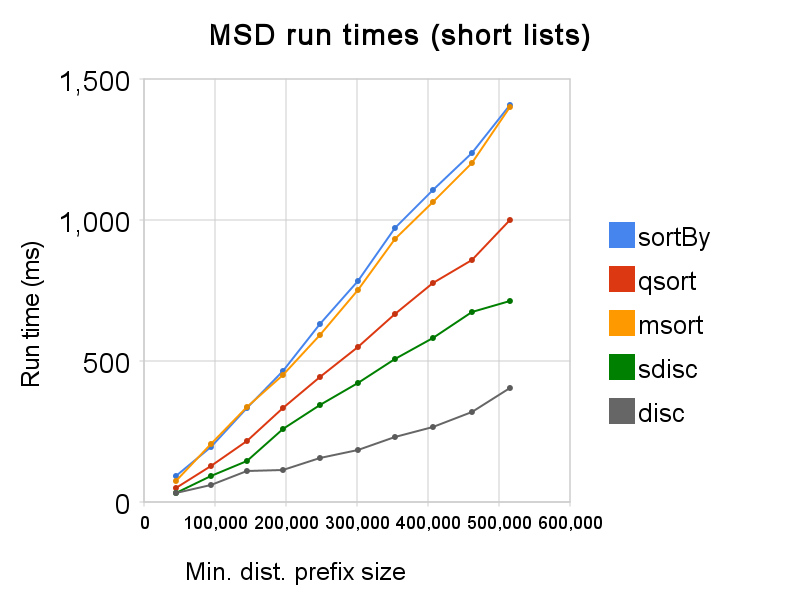
\includegraphics[width=\textwidth]{figures/msd-short-lists}
\end{frame}

\begin{frame}{Performance}
  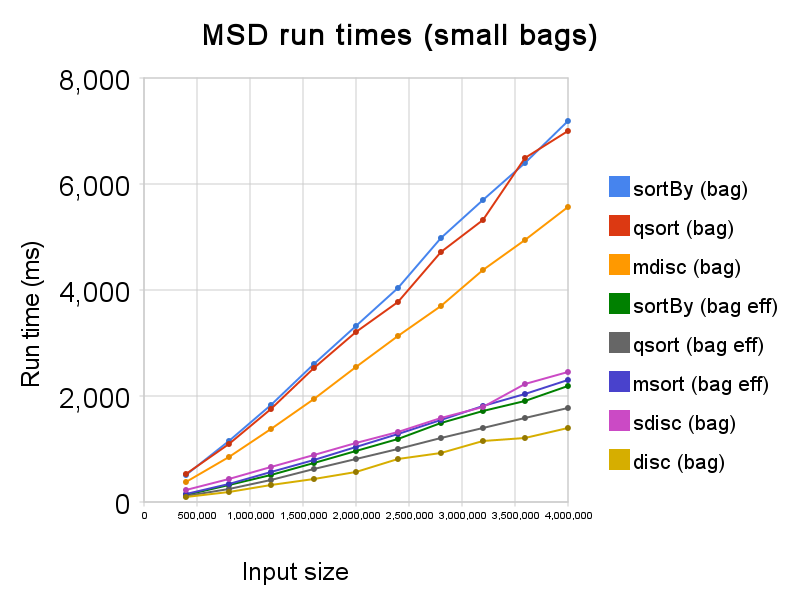
\includegraphics[width=\textwidth]{figures/msd-small-bags-all}
\end{frame}

\begin{frame}{Performance}
  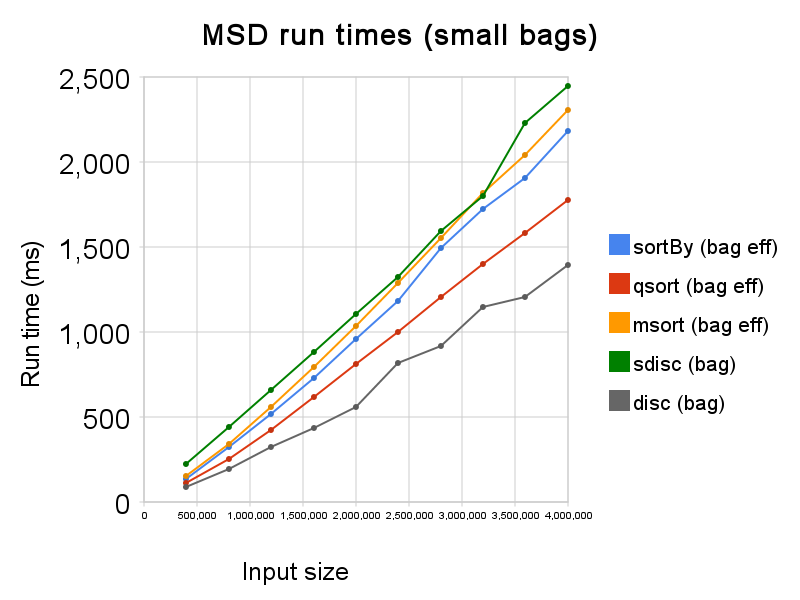
\includegraphics[width=\textwidth]{figures/msd-small-bags}
\end{frame}

\begin{frame}{Performance}
  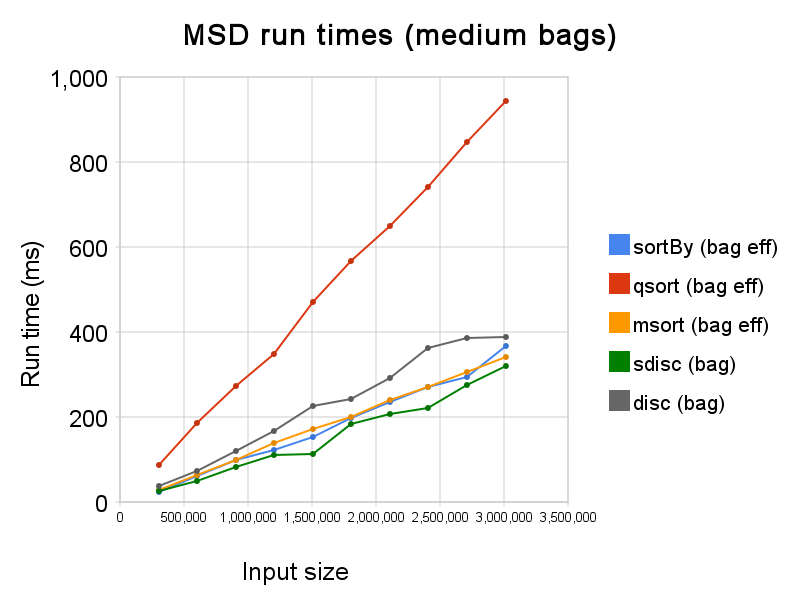
\includegraphics[width=\textwidth]{figures/msd-medium-bags}
\end{frame}

\begin{frame}{Performance}
  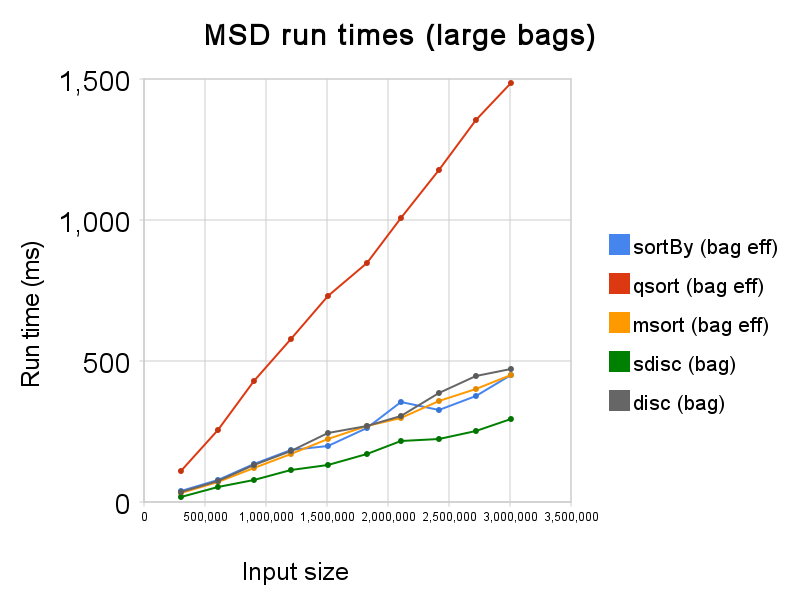
\includegraphics[width=\textwidth]{figures/msd-large-bags}
\end{frame}

\begin{frame}{Variations, extensions}
  \begin{itemize}
  \item Domain-theoretic semantics
  \item Avoiding sparse bucket table traversals for order discrimination and
    sorting
  \item Equivalence expressions (analogous to order expressions)
  \item Bag and set equivalence discrimination
  \item Run-time order and equivalence normalization for correctness and
    efficiency
  \item Combinatory discriminator library (without order/equivalence
    expressions, requires rank-2 polymorphic types)
  \item Comparison with complexity of sorting
  \item Generic tries
  \item Nontrivial applications: AC-term equivalence, type isomorphism,
    \textbf{equijoins}
  \end{itemize}
\end{frame}

\begin{frame}{Select related work}
  \begin{itemize}
  \item Paige et al. (1987-97): Basic multiset discrimination for pointers,
    strings, acyclic graphs; application to lexicographic sorting
  \item Henglein (2003): Unpublished note on multiset discrimination
    (top-down, bottom-up) and algorithms for circular data structures
  \item Ambus (MS thesis, 2004): Java discriminator library, internal and
    external (disk) data, application to asynchronous data coalescing in
    P2P-based XML Store (see plan-x.org)
  \item Henglein (ICFP 2008): Order discriminators
  \item Henglein (JFP, Nov.\ 2012): \emph{Generic top-down discrimination
      for sorting and partitioning in linear time}
  \item Henglein, Hinze (APLAS 2013): Generic Sorting and Searching
  \item Kmett (2015): Generic discrimination, streaming
  \end{itemize}
\end{frame}

\begin{frame}{Open problems (``Homework'')}
  \begin{itemize}
  \item Generic bottom-up discrimination (for acyclic data structures)
  \item Generic cyclic discrimination (for cyclic data structures)
  \item Staged implementation (partial evaluation)
  \item Parallel discrimination
  \end{itemize}
\end{frame}

\begin{frame}{Take-home message: GAS}
  Simultaneously:
  \begin{itemize}
  \item \textbf{Genericity:} DSL for orders and equivalences for correctness
    and safety/limited expressiveness
  \item \textbf{Abstraction:} Statically guaranteed representation
    independence
  \item \textbf{Scalability:} Asymptotically optimal computational
    performance
  \end{itemize}
  \emph{All equi-abstract interfaces are equivalent, but some are faster than
    others.}
\end{frame}

\begin{frame}{Program}
  \begin{enumerate}
  \item Today: Generic discrimination
  \item Generic multiset programming
  \item Generic linear algebra
  \end{enumerate}
  \vspace{1cm}
  \begin{center}
    End of talk
  \end{center}
\end{frame}

\end{document}
